\documentclass{article}
\usepackage{graphicx}
\usepackage{hyperref}
\title{Offline dictionary attack\\
	 \large \\ HW2 - CNS Sapienza}
\author{Giulia Muscarà 1743261} 
\date{November 14, 2019} 

\begin{document}
\maketitle

\section{Objectives}
The purpose of this report was to carry out an offline dictionary attack to decrypt a given ciphertext and some additional information about it. The encryption was made by the following given command. \\ \\
\textbf{openssl enc -aes-192-cbc -pbkdf2 -e -in plaintext.txt -out ciphertext.enc}\\ \\
The option -pbkfd2 creates a hex-encoded derived key from the password used for the encryption.
The plaintext originally was a text made of english language words and the password to find was a meaningful word.

\section{Approach}
To carry out the analysis, Python was chosen as it is a powerful high-level programming language for technical computing. The version of OpenSSL that was adopted is the 1.1.1d. \\ 
Knowing that the plaintext was made of english language words and that the password to find was a meaningful word, the word list chosen to carry out the first trial of attack was an english word list, as it was likely that a text file written in english was encrypted by an english speaking person.
As a first attempt, the wordlist used was entirely made of lowercase words, to use an upper case list only in the case this strategy would not have been successful. \\
The dictionary was downloaded from \href{http://www.gwicks.net/dictionaries.htm
}{JUST WORDS!}, a website with a wide range of dictionaries and word lists in qtyp dictionary and simple text formats. The file was not attached because of its dimension but the previous link redirects directly to the download page. The chosen wordlist is of 194,000 english lowercase words and was put in a .dic file format, as shown un Fig. 1.\\ 

\clearpage

\begin{figure}[t]
	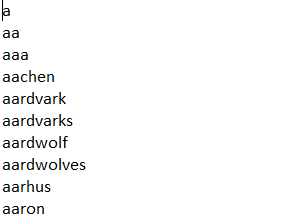
\includegraphics{img1-hw2-1743261.png}
	\caption{Wordlist format}
\end{figure}

With the words being separated only by a newline, it was possible to open and read it using the open("english.dic", "r") python function and then to parse the words using the newline as delimiter.
For each word in the list, the subprocess module was used, allowing to spawn a new process, connect to its input, output and error pipes, and to obtain its return code. The process invoked was the openssl decryption command, trying the current word as decryption password. In the case the trial was successful and the password was found, the output plaintext was printed on the "plaintext-hw2-1743261.txt" file. \\
To record the running time necessary to find the password, the time module was adopted. In particular the function timeit() provides a simple way to time specific parts of the Python code, so as to measure the sum of the times to try all the different words before finding the right one. The found password and the total time taken by the process were printed, as shown in the following figure.\\

\begin{figure}[h]
	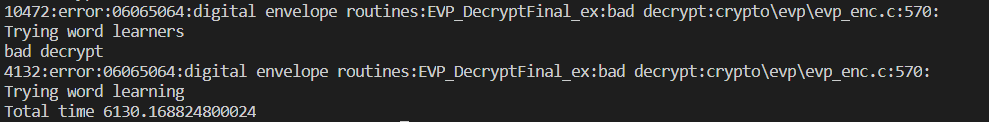
\includegraphics[width=1\textwidth]{img2-hw2-1743261.png}
	\caption{Output}
\end{figure}

\section{Conclusion}
The password "learning" was found after 6130.169 seconds. The plaintext was consequently output on the "plaintext-hw2-1743261.txt" file. The content of the original file was an extract from Shakespeare's "Hamlet". This shows that the symmetric key derived from the password was vulnerable to a dictionary attack, that was successfully conducted.

\end{document}